\documentclass[aspectratio=169]{beamer}

\usetheme{Madrid}
\usecolortheme{default}
\setbeamertemplate{navigation symbols}{}
\setbeamertemplate{footline}[frame number]

\usepackage{amsmath,amssymb}
\usepackage{tikz}
\usetikzlibrary{arrows.meta,positioning,decorations.pathreplacing}
\usepackage{booktabs}
\usepackage{xcolor}

\title[Digital Signatures]{Digital Signatures}
\subtitle{Number-Theoretic Foundations and Applications}
\author{}
\date{\today}

\begin{document}

\frame{\titlepage}

\begin{frame}{Outline}
\tableofcontents
\end{frame}

%================================================
\section{Motivation}
%================================================
\begin{frame}{What Problem Are We Solving?}
\begin{block}{Goal}
Given a message $m$ and a private key, produce $\sigma$ such that \emph{anyone} with the public key can confirm:
\end{block}
\begin{itemize}
    \item \textbf{Authenticity} --- only the key owner could have produced $\sigma$
    \item \textbf{Integrity} --- any change to $m$ breaks verification
    \item \textbf{Non-repudiation} --- the signer can't later deny it
\end{itemize}
\vspace{0.3cm}
\centering
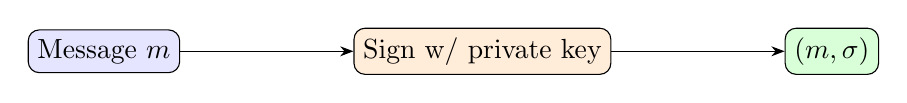
\begin{tikzpicture}[node distance=1.6cm, >=Stealth]
\node[draw, rounded corners, fill=blue!10] (m) {Message $m$};
\node[draw, rounded corners, fill=orange!15, right=2.2cm of m] (sign) {Sign w/ private key};
\node[draw, rounded corners, fill=green!15, right=2.2cm of sign] (sig) {$(m,\sigma)$};
\draw[->] (m) -- (sign);
\draw[->] (sign) -- (sig);
\end{tikzpicture}
\end{frame}

%================================================
\section{Number Theory Toolkit}
%================================================
\begin{frame}{The Group $\mathbb{Z}_n^*$}
\begin{itemize}
    \item $\mathbb{Z}_n^* = \{a \in \{0,\dots,n-1\} : \gcd(a,n)=1\}$
    \item Forms a group under multiplication mod $n$, order $\varphi(n)$
    \item If $n = p$ prime: $\varphi(p) = p-1$
    \item If $n = pq$, distinct primes: $\varphi(n) = (p-1)(q-1)$
\end{itemize}
\vspace{0.3cm}
\begin{exampleblock}{Why we care}
This group structure is the entire ``state space'' RSA arithmetic lives in.
\end{exampleblock}
\end{frame}

\begin{frame}{Fermat \& Euler: The Two Load-Bearing Theorems}
\begin{block}{Fermat's Little Theorem}
$p$ prime, $p \nmid a$ $\implies$ $a^{p-1} \equiv 1 \pmod p$
\end{block}
\begin{block}{Euler's Theorem}
$\gcd(a,n) = 1$ $\implies$ $a^{\varphi(n)} \equiv 1 \pmod n$
\end{block}
\vspace{0.2cm}
\centering{\Large Everything RSA does is exploit this single congruence.}
\end{frame}

\begin{frame}{Discrete Logarithm Problem}
\begin{columns}
\column{0.55\textwidth}
\begin{itemize}
    \item Cyclic group $G$, generator $g$, order $q$
    \item \textbf{Easy}: given $x$, compute $g^x$ (repeated squaring, $O(\log x)$)
    \item \textbf{Hard}: given $h=g^x$, recover $x$
    \item No efficient classical algorithm known in $\mathbb{Z}_p^*$ or elliptic curve groups
\end{itemize}
\column{0.45\textwidth}
\centering
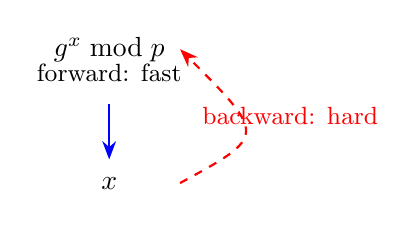
\begin{tikzpicture}[>=Stealth]
\node at (0,1.4) {\small forward: fast};
\draw[->, thick, blue] (0,1) -- (0,0.3);
\node at (0,0) {$x$};
\node at (0,1.7) {$g^x \bmod p$};
\draw[->, thick, red, dashed] (0.9,0) .. controls (2,0.6) .. (0.9,1.7);
\node at (2.3,0.85) {\small \textcolor{red}{backward: hard}};
\end{tikzpicture}
\end{columns}
\end{frame}

%================================================
\section{RSA Signatures}
%================================================
\begin{frame}{RSA: Key Generation}
\begin{enumerate}
    \item Pick large primes $p, q$; let $n = pq$
    \item $\varphi(n) = (p-1)(q-1)$
    \item Pick $e$ with $\gcd(e,\varphi(n))=1$
    \item Solve for $d \equiv e^{-1} \pmod{\varphi(n)}$
\end{enumerate}
\vspace{0.2cm}
\begin{alertblock}{Keys}
Public: $(n,e)$ \hspace{1cm} Private: $d$
\end{alertblock}
\end{frame}

\begin{frame}{RSA: Sign and Verify}
\[
\textbf{Sign: } \sigma \equiv m^{d} \pmod n
\qquad\qquad
\textbf{Verify: } \sigma^{e} \bmod n \stackrel{?}{=} m
\]
\vspace{0.4cm}
\begin{theorem}
$(m^d)^e \equiv m \pmod n$ for all $m \in \mathbb{Z}_n^*$.
\end{theorem}
\textbf{Proof sketch:} $ed = 1 + k\varphi(n)$ for some integer $k$, so
\[
(m^d)^e = m^{1+k\varphi(n)} = m \cdot (m^{\varphi(n)})^k \overset{\text{Euler}}{=} m \cdot 1^k = m.
\]
\end{frame}

\begin{frame}{RSA: Fully Worked Example}
\[
p=61,\ q=53 \;\Rightarrow\; n = 3233,\ \varphi(n) = 3120
\]
\[
e = 17 \;\Rightarrow\; d = 2753 \quad (17\times 2753 = 46801 = 15\times3120+1)
\]
\vspace{0.2cm}
\textbf{Sign $m = 65$:}
\[
\sigma = 65^{2753} \bmod 3233 = 2790
\]
\textbf{Verify:}
\[
2790^{17} \bmod 3233 = 65 \; \checkmark
\]
\begin{alertblock}{Tamper test}
Flip $m \to 66$: verification gives $65 \neq 66$ --- rejected!
\end{alertblock}
\end{frame}

\begin{frame}{Live Demo}
\centering
\Large
Let's generate keys, sign, and verify live. \\[0.4cm]
\normalsize
Call out two small primes and a message number --- \\
we'll watch the arithmetic resolve on screen.
\vspace{0.5cm}

\textit{(Switch to the interactive RSA signature tool now.)}
\end{frame}

%================================================
\section{Discrete-Log Signatures}
%================================================
\begin{frame}{ElGamal Signatures}
Public key $y = g^x \bmod p$; private key $x$.
\vspace{0.2cm}
\textbf{Sign} (pick random ephemeral $k$, $\gcd(k,p-1)=1$):
\[
r = g^k \bmod p, \qquad s = (m - xr)k^{-1} \bmod (p-1)
\]
\textbf{Verify:}
\[
g^{m} \stackrel{?}{\equiv} y^{r} r^{s} \pmod p
\]
\begin{alertblock}{Critical rule}
Never reuse $k$! Reuse leaks $x$ instantly via linear algebra.
\end{alertblock}
\end{frame}

\begin{frame}{DSA and ECDSA}
\begin{itemize}
    \item \textbf{DSA}: works in a prime-order subgroup of $\mathbb{Z}_p^*$ $\to$ shorter signatures
    \item \textbf{ECDSA}: replaces $\mathbb{Z}_p^*$ with points on an elliptic curve $E(\mathbb{F}_p)$
    \item Same underlying idea: DLP hardness, just in a different group
\end{itemize}
\vspace{0.3cm}
\begin{table}
\centering
\begin{tabular}{lcc}
\toprule
 & 128-bit security & Signature size \\
\midrule
RSA & 3072-bit $n$ & large \\
ECDSA & 256-bit curve & small \\
\bottomrule
\end{tabular}
\end{table}
\end{frame}

%================================================
\section{Applications}
%================================================
\begin{frame}{Where This Shows Up Every Day}
\begin{itemize}
    \item \textbf{TLS/HTTPS} --- certificate chains signed by CAs
    \item \textbf{Code signing} --- OS/app-store update verification
    \item \textbf{Blockchain} --- every Bitcoin/Ethereum transaction is ECDSA-signed
    \item \textbf{e-Government \& PDF signing} --- legal non-repudiation
    \item \textbf{Software supply chain} --- PGP/GPG, Sigstore
\end{itemize}
\end{frame}

%================================================
\section{Conclusion}
%================================================
\begin{frame}{Takeaways}
\begin{itemize}
    \item Digital signatures = number theory with a trapdoor
    \item RSA: security from factoring; correctness from Euler's theorem
    \item ElGamal/DSA/ECDSA: security from discrete logs
    \item Elliptic curves buy the same security with far smaller keys
    \item The math you just saw runs behind every HTTPS padlock and blockchain transaction
\end{itemize}
\vspace{0.4cm}
\centering \Large Questions?
\end{frame}

\end{document}
